\documentclass{ctexart}

\title{软件工程}

\usepackage{graphicx}

\begin{document}
\maketitle

\section{介绍}
\paragraph{生命周期地看待} 软件不是写完就完了, 而是需要持续的维护.
\paragraph{过程评估} 即使软件没有完成, 也可以在过程中评估软件.
\pagebreak{项目产出} 项目的产出除了可用的程序, 还有如文档.
\paragraph{人月神话} 软件开发中, 不是人越多就开发越快, 相反可能更多的中途加入的人会拉慢进度.
\paragraph{开发和客户交流} 客户需要不断的和开发交流, 以修正轨迹和提供更精确的方向指导.

\section{持续集成和git}
    系统可能随时变化, 预测式的开发已经不合时宜了.

\section{代码风格}


\pagebreak
\section{重构}
    \begin{figure}[ht!]
        \centering
        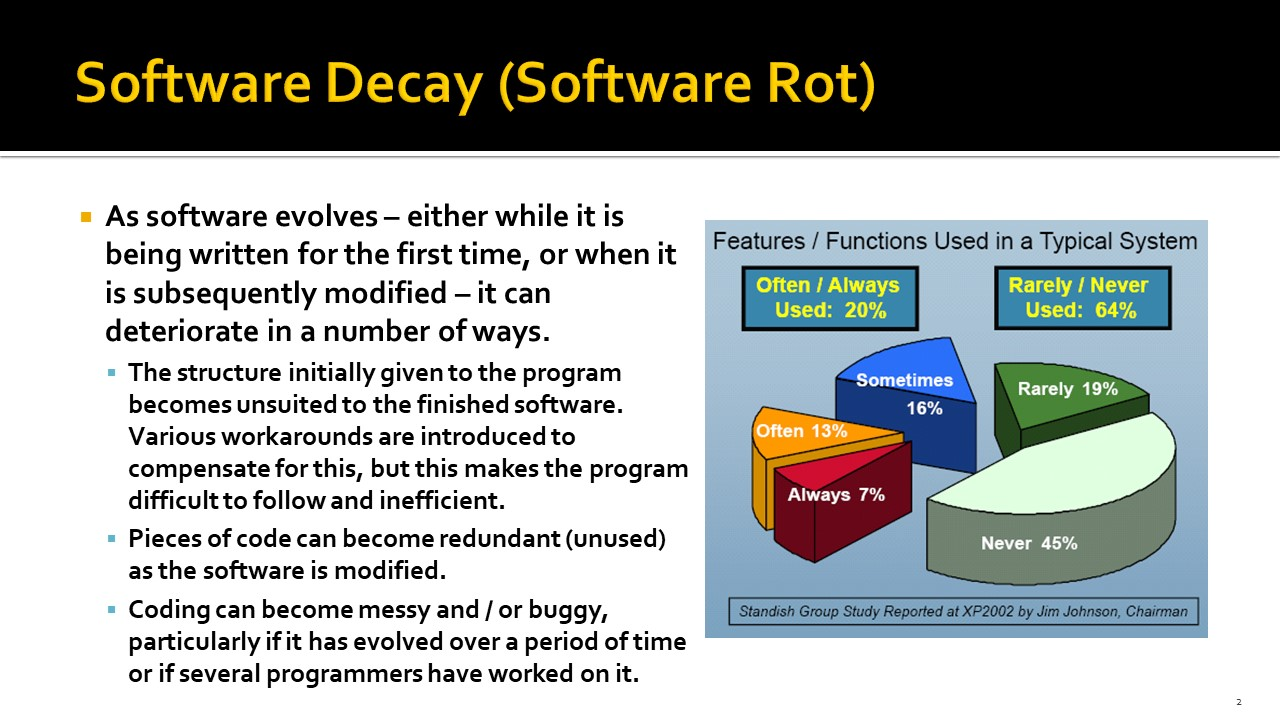
\includegraphics[width=\textwidth, height=\textheight, keepaspectratio]{refactor-1.jpg}
        \caption{Software Rot现象}
    \end{figure}

    \begin{figure}[ht!]
        \centering
        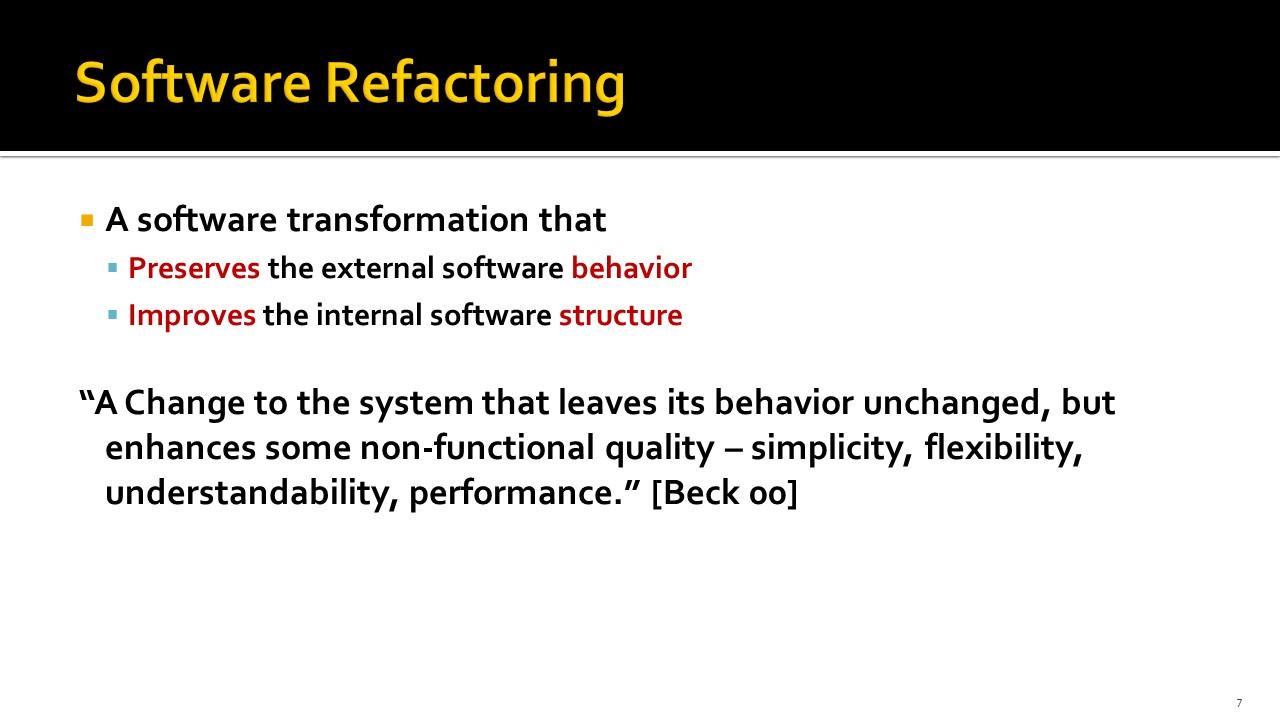
\includegraphics[width=\textwidth, height=\textheight, keepaspectratio]{refactor-2.jpg}
        \caption{何谓Refactoring}
    \end{figure}

    \begin{figure}[ht!]
        \centering
        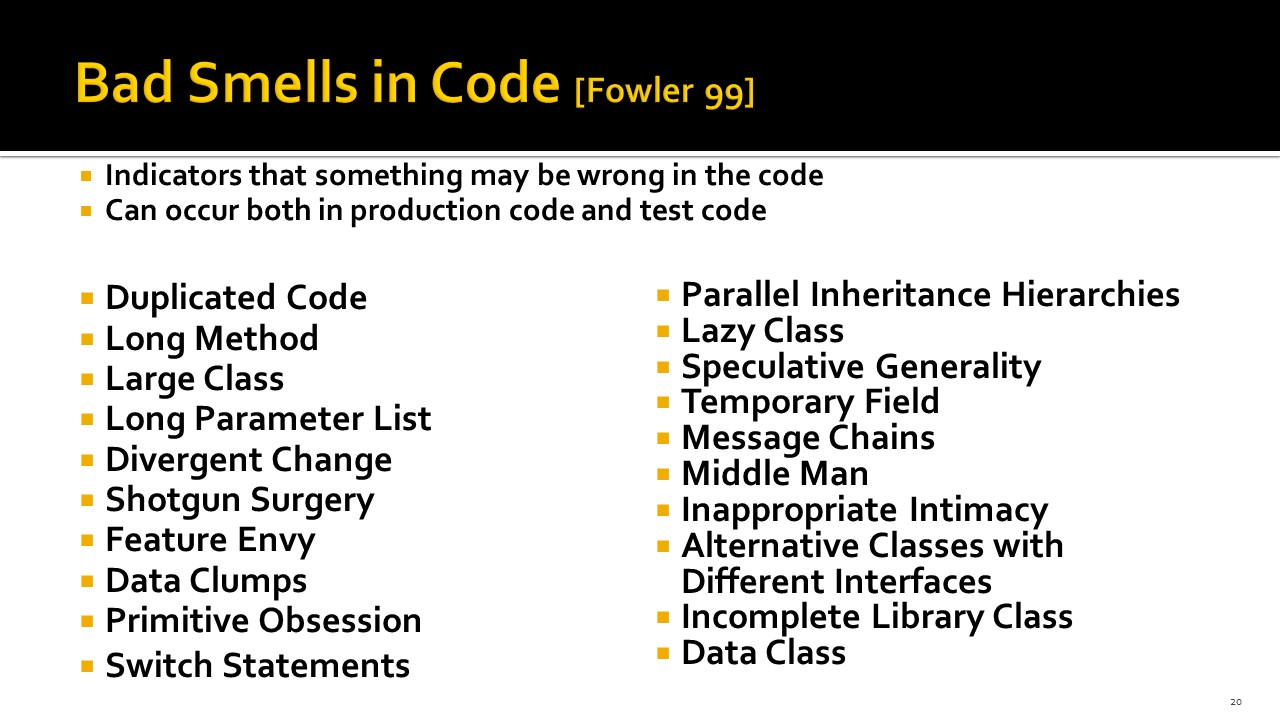
\includegraphics[width=\textwidth, height=\textheight, keepaspectratio]{refactor-3.jpg}
        \caption{常见的Code Smell}
    \end{figure}

    \begin{figure}[ht!]
        \centering
        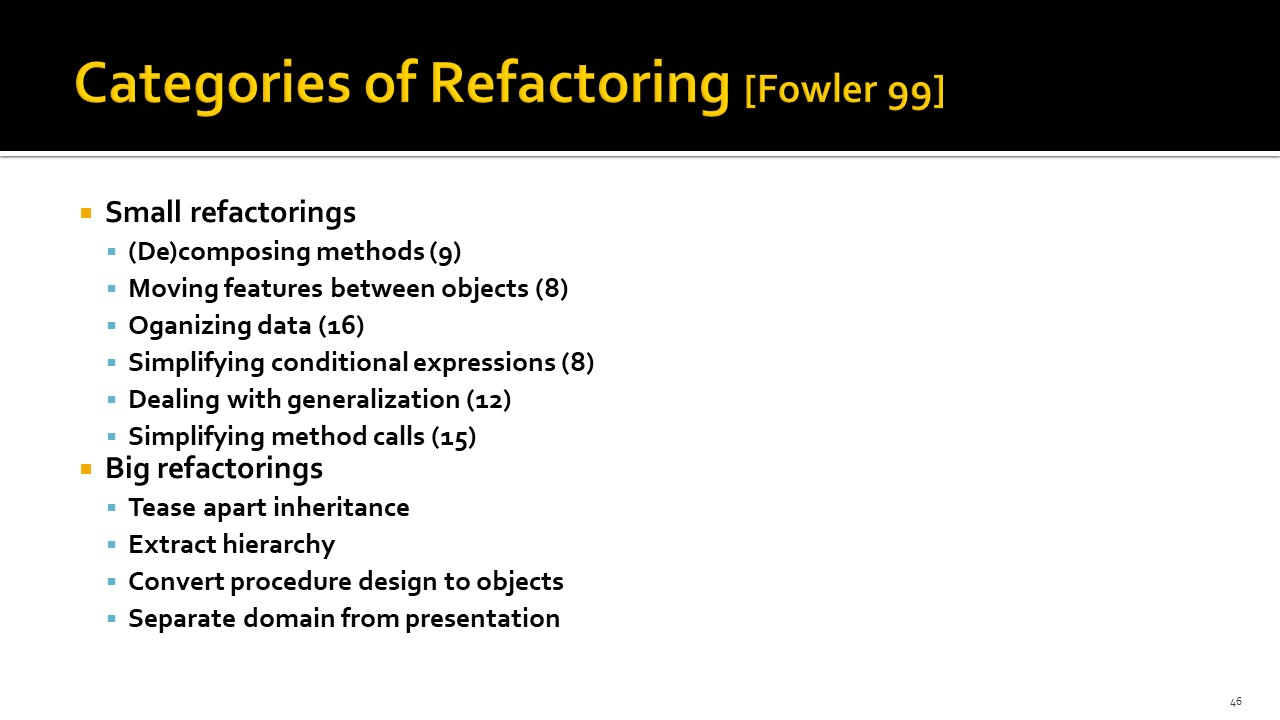
\includegraphics[width=\textwidth, height=\textheight, keepaspectratio]{refactor-4.jpg}
        \caption{常见的Refactor方法}
    \end{figure}

\section{测试}
    测试: 希望找到错误.
    好的测试是容易找到错误的测试.\par
    基本原则是, 测试是不可穷尽的.
\paragraph{测试样例} 指定输入, 输出, 以及可能的执行前置条件etc.
\subsection{分类}
    \begin{description}
        \item[白盒测试] 已知要测试的代码. 是基于代码测试的, 测试功能是代码的子集.\\
            包含控制流覆盖率和数据流覆盖率;
        \item[黑盒测试] 已知要测试的特性, 是基于规格测试的, 测试功能是规格的子集.\\
            包含需求覆盖率
    \end{description}
    考虑测试韦恩图, 有集合$S$表示规格, $P$表示程序, $T$表示测试.
    白盒测试是$T \subseteq P$; 黑盒测试是$T \subseteq S$.
\subsection{控制流测试}
\paragraph{Statement Coverage}
    C0测试; 所有语句都必须被测试覆盖.\par
    方法: 在控制流图中找到覆盖所有语句 (即覆盖所有节点) 的路径 (可能的话需要路径集合), 寻找输入适配此路径.
\paragraph{Decision Coverage}
    C1测试; 所有if语句的条件必须测试过true和false.\par
    方法: 寻找覆盖所有分支 (每个节点的每条出边必须被覆盖) 的路径集合, 寻找输入适配路径集合.
\paragraph{Predicate Converage}
    C1P测试; 所有if语句的条件中每个原子条件必须测试过true和false.\par
    方法: 将if的复合条件改写成嵌套if之后看.
\paragraph{Multiple Condition Coverage}
    CMCC测试; \emph{每个复合条件}中所有原子条件的组合都被测试. 组合会有依赖关系所以不一定是$2^n$种路径.\par
    方法: 同C1P测试, 只是需要更多路径.
\paragraph{All Path Coverage}
    C$\infty$测试; \emph{整个程序}中所有原子条件的组合都被测试, 即所有路径都被测试.\par
    通常在有循环时时不可行的, 或者在条件互斥时也不可行 (某一条路径不存在对应的输入).
\paragraph{cyclomatic complexity (McCabe complexity)}
    覆盖所有控制语句 (C0测试) 需要的最少的测试例数. 其等于流图中, 决策的数量加1.
\paragraph{Independent Path}
    有向图中的独立路径. 数目等于 cyclomatic complexity.

\subsection{数据流测试}
    不正常的数据行为: \begin{itemize}
        \item (dd) 定义之后, 引用前重定义
        \item (ur) 未定义时引用
        \item (du) 定义后未引用
    \end{itemize}
    数据流分析分为静态和动态, 以是否执行原代码为准.
\paragraph{DU链} $[X, S, S']$的形式, $S$, $S'$是语句,
    $S$定义而$S'$引用$X$, 并且$S$的定义在$S'$是存活的.
\paragraph{数据流图} 将数据的引用分为计算引用 (C-uses) 和条件引用 (P-uses),
    基本结构类似流图, 但是结点是计算引用, 边与条件引用挂钩.
\paragraph{覆盖度量} 包含 All paths (通常不可能),
    All DU paths, All Edges (通常最低要求)等.

\subsection{黑盒测试}
\paragraph{基本思想} 将输入空间分成多个等价类, 每个等价类对于程序来说是等价的, 从``发现错误''的角度.
\paragraph{强弱测试} 强测试即, 可能有多个无效的输入, 弱测试即, 只有一个输入时无效的.
\paragraph{普通鲁棒测试} 普通测试只覆盖有效数据, 鲁棒测试还覆盖无效数据.\par
    普通鲁棒测试和强弱测试都是EP测试.
    \begin{figure}[ht!]
        \centering
        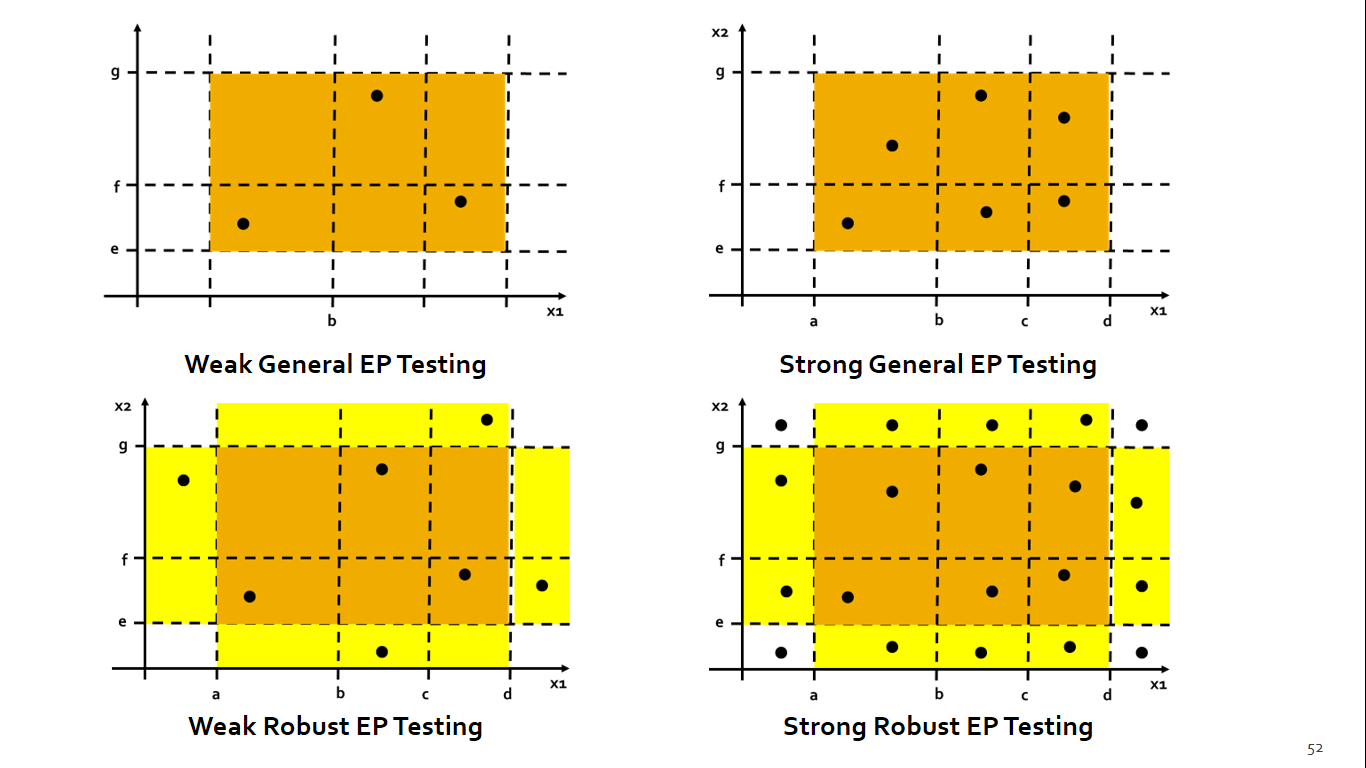
\includegraphics[width=\textwidth, height=\textheight, keepaspectratio]{eptest.png}
        \caption{EP测试的例子}
    \end{figure}

\paragraph{边界值分析} 通常问题都是在输入在输入域边界时出现的.
    因此, 选择数据时, 不是随机在数据空间选择, 而是在空间边界选择.
    同时也从输出域中寻找数据.\par




\end{document}
